\chapter{Pose Estimation Development}
\label{chapter4}

\section{RGB-to-RGBD}

Multiple methods were discussed to solve the human-robot distance task. Two of these, used the RGB-D sensory data which comes integrated on TIAGO, while the third one made use of laser readings incoming from the range-finder sensor also available on TIAGO.

From a point of view of user reachability, it would have made sense to use the triangulation method as most robotics systems nowadays are equipped with cameras for their perception. Moreover, the availability of fully functional triangulation routines in OpenCV, would have made the implementation of the triangulated solution straightforward. Such approach, however, requires a stereo or binocular vision system, which consists in having two cameras close to each and registered to one another, thereby finding the depth solving the system of linear equations previously presented. However, this was not the case, as TIAGO has only a monocular vision system incorporated with a depth sensor.

Another viable solution was to use the cob\_leg\_detection \cite{website:cobLegDetection} package available in ROS. The method makes use of laser-scan readings to find people's legs in the environment, which proved to be extremely sensible to false positives especially in cluttered areas, where tables and chairs were detected as people. Possibly the PCL\footnote{Point Cloud Library} library and its RGB-D HOG based implementation for people detection \cite{munaro2014fast} could have been used, however, similarly to the plain RGB HOG introduced in chapter2, only people in up-right positions were effectively detected, which did not make sense to use especially when a more reliable and sophisticated method such as the RGB person recognition was available.

Therefore it was decided to use the integrated RGB-D camera and the already available depth-map with per-pixel distance. This overall was a better development choice, as it reduced the implementation time given that no added routine or logic were needed as well as the computational costs given that only a depth-image conversion and RGB to depth pixel correspondence were actually needed to obtain a an accurate distance estimation.

\section{Development Phases}

The overall pose retrieval logic was split into two phases, a depth one and a pose one. The depth phase uses the detection module results and finds the corresponding detection's bounding-box centre point in the depth-image, hence obtaining the resulting person-robot distance for each detection in the collection. The pose phase uses the computed distances to compute the 3D map pose for each detection, therefore a map coordinate frame has to be available.

\section{Depth Phase}

The depth computation is implemented as a function called \textbf{getPoses} found in the \textbf{pose\_finding.py} script. The routine takes as an argument a ROS service request, which includes two inputs, the detection module message and the synchronised raw depth-image with the raw colour-image. The steps taken in the depth phase are the following:

\begin{enumerate}
  \item Image conversion
  \item Distance computation
  \item Message publication
\end{enumerate}

\subsection{Image conversion}

Similarly to what was done in the conversion module and its raw colour-image conversion into an OpenCV format is repeated in the pose component. In fact, the passed depth-image is a ROS standard\_msg/Image type, that holds 32bits raw floating point values which are nowhere near the required metre values for the computation. Hence, another conversion is made using the same \textbf{imgmsg\_to\_cv2} routine which however in this case is converted to a \textbf{32FC1} encoding rather then a \textbf{BGR8}. The converted image obtained consists in a numpy array where each entry is 1:1 mapped every RGB pixel stores the corresponding distance value in metres as one channel floating point with single precision. The conversion is as follows:

\begin{lstlisting}
# Convert depth-image into a float32 array of metre values
cv_depth_image = CvBridge().imgmsg_to_cv2(depth_raw_image, '32FC1')
\end{lstlisting}

\subsection{Distance Computation}

The computation consists in merging the detection module data with the converted depth-image. In fact, by knowing with confidence the centre point for each detection, in terms of its x and y coordinate, these can be used to access the corresponding distance within the depth-image. RGB-D measurements, like any other sensor, are subject to noise and therefore an average distance is computed over the neighbouring pixels of the centre coordinate, called ROI\footnote{Region of Interest}. Therefore allowing allowing a more robust distance estimation.

The ROI extraction process makes use of three variables: \textbf{d}, \textbf{x}, and \textbf{y}. The variable d is the size of the neighbours around the centre point or how far shall the ROI look into to compute the average distance, while the x and the y are the detection's bounding box centre point.

The previously converted depth-image is used to fetch all the values \textbf{d} away from the centre point using Python's slicing feature that enables the retrieval of values within an array, in this case a numpy array, by using simple range indexing. The ROI obtained however, is still not ready to be used, as it might contain invalid values, due to the light beam hitting particular textures or just for being outside of the sensor range, which would make the computation fail. Hence numpy's \textbf{np.isnan} functionality is used along with the negation feature \textbf{~} to strip away from the array all invalid values, which in this case occur to be defined as NaN. The result from the stripping process is then used to compute the average distance by using the \textbf{sum} and \textbf{size} routines from numpy's library to get the distance by dividing the array's elements sum by its size as follows:

\begin{lstlisting}
# Retrieve the ROI
roi = cv_depth_image[j-d:j+d+1, i-d:i+d+1]
    
# Filter invalid NaN values
roi = roi[~np.isnan(roi)]
    
# Compute average distance
average_distance = np.sum(roi) / roi.size
\end{lstlisting}

\subsection{Publish distances}

The computed distance for each detection are published over a topic called \textbf{distances} created using the \textbf{Publisher} routine available through the rospy library that publishes custom \textbf{Distances} messages. The function arguments are the topic's name, in this case distances, the message type which a custom created message called Distances and buffer size queue as follows:

\begin{lstlisting}
self.distance_pub = rospy.Publisher('distances', Distances, queue_size=5)
\end{lstlisting}

In fact, two custom messages were created for the publishing process and added to the msg folder at the root of the package. These are the \textbf{Distance.msg}, which holds the distance value for every single detection and the \textbf{Distances.msg} one that stores the collection of Distance messages for each detection. The two message definitions for the Distance.msg(left) and the Distances.msg(right) are shown below:

\begin{multicols}{2}
  \begin{itemize}
    \item int32 ID
    \item float32 depth
  \end{itemize}

  \columnbreak

  \begin{itemize}
    \item Header header
    \item Distance[] array
  \end{itemize}
\end{multicols}

The Distance message fields are two. A 32bits integer values storing the same ID of the detection which distance was computed so as to recognise which distance is to which detection, and a 32bits floating point values that contains the distance values in metres of the detection. The Distances message has as well two fields, a header with the timestamp information of the message creation and a list of Distance type that aims at storing the single Distance object for every detection processed. Similarly to the Detection and Detections messages, the Distance and Distances messages need to be added to the CMAKE file and built using catkin build to be available for usage within the package.

To populate the messages and to carry the distance computation for the passed detections, a for loop statement is used that loops over the Detections' array field where a Distance instance is created at every iteration and populated. Every instance is then pushed to the Distances instance declared at the top of the function using the append routine on its array field.

\begin{figure}[H]
  \begin{center}
    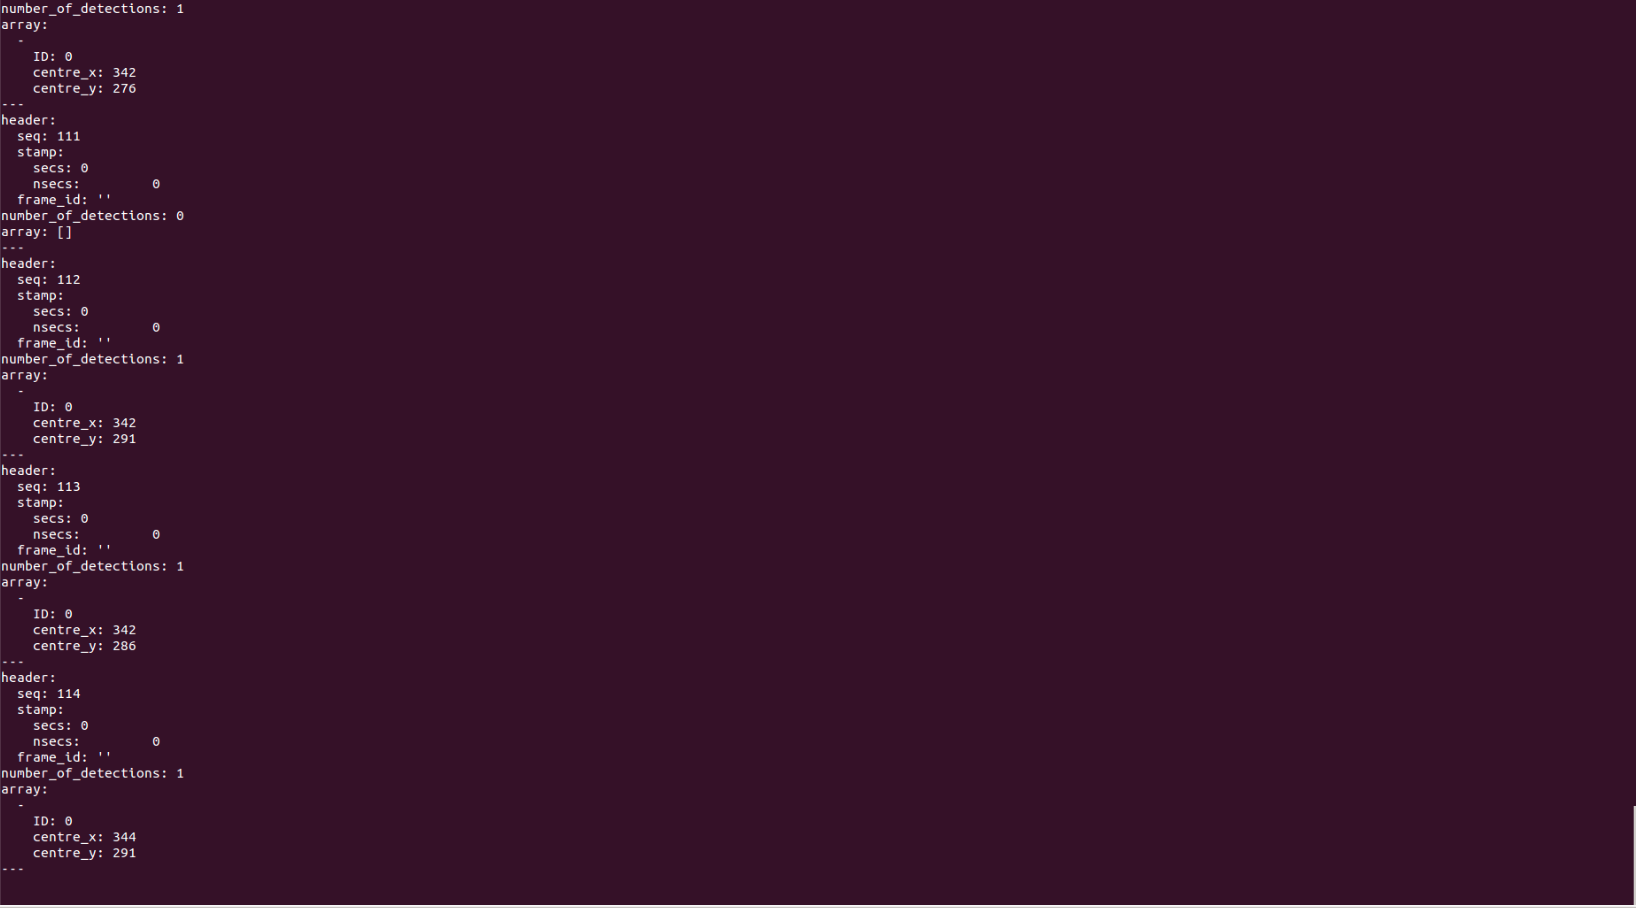
\includegraphics[width=.8\linewidth]{images/chapter3_detections_topic.png}
  \end{center}
  \caption{Distances topic output.}
  \label{fig:distance_topic}
\end{figure}

\subsection{Ratio offset}

The 3D pose estimation process is such that it forms a chain, as the depth module make use of the detection's module output, and the depth computed in the distance module is used by the pose component to back-projection the centre pixel point and transform it in the space. Therefore, a mistake at an early stage would cause the error to propagate through the chain.

The initial detection stage, that makes use of the neural network for the person detection, takes as input a 300x300 pixel resolution due to the architecture of the network. However, the depth-image obtained after the conversion has a resolution of 640x480 pixels, meaning that the assumed 1:1 mapping of the centre location of the bounding box (computed on the 300x300 RGB image) is invalid, as the two resolutions are different. This circumstance was not taken into consideration at first and brought some meaningful errors in the distance computation as the wrong ROI was indexed in the converted depth-image and therefore the wrong distance values were used as shown in the images below.

\begin{figure}[H]
	\centering
    \begin{subfigure}{.6\textwidth}
      \centering
      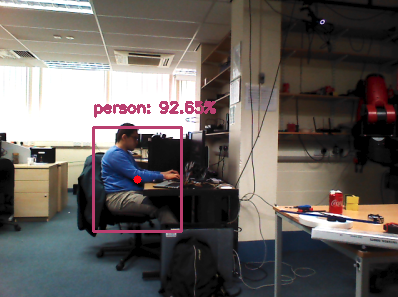
\includegraphics[width=8cm]{images/chapter4_rgb_ratio.png}
      \caption{RGB detection.}
      \label{fig:ratin}
    \end{subfigure}%
    
    \begin{subfigure}{.6\textwidth}
      \centering
      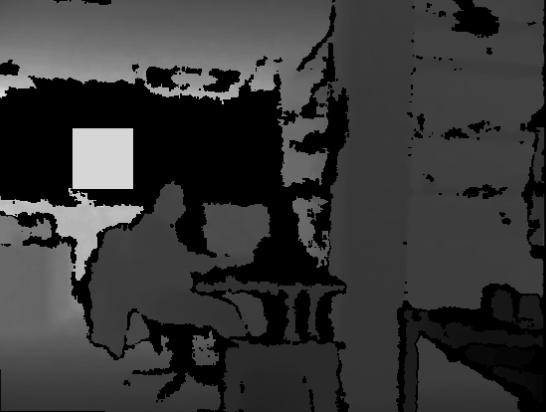
\includegraphics[width=8cm]{images/chapter4_rgbd_no_ratio.png}
      \caption{Depth image with ROI drawn (the white box).}
      \label{fig:ration}
    \end{subfigure}%
    
    \caption{Ratio offset between the actual centre point and the ROI.}
\end{figure}
\clearpage

The solution to the problem consisted in using ratios to find the corresponding centre point of the bounding box in the 300x300 image within the 640x480 depth-image. Hence given the x and y coordinates of the centre point, where x represents the width of the image and y its height, the respective coordinates in the 640x480 depth-image resolution become:

\[x640 = (x/400) * 640 \]
\[y480 = (y/300) * 480 \]

and by converting each detection's centre point prior to the depth module call using the defined \textbf{getRatio} function, a correct ROI is obtained as shown below.

\begin{figure}[H]
	\centering
    \begin{subfigure}{.5\textwidth}
      \centering
      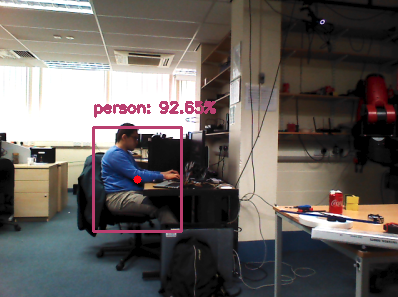
\includegraphics[width=8cm]{images/chapter4_rgb_ratio.png}
      \caption{RGB detection.}
      \label{fig:ratin}
    \end{subfigure}%
    
    \begin{subfigure}{.5\textwidth}
      \centering
      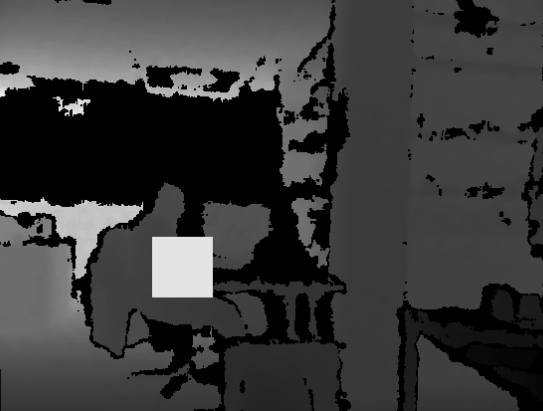
\includegraphics[width=8cm]{images/chapter4_rgbd_ratio.png}
      \caption{Depth image with ROI drawn (white box).}
      \label{fig:ration}
    \end{subfigure}%
    
    \caption{Correct point correspondence between the actual centre point and the ROI.}
\end{figure}

\section{Pose phase}

The pose phase where the actual 3D map location for every detection is found has three different steps, below outlined:

\begin{enumerate}
  \item Image plane projection
  \item 3D conversion
  \item Markers \& message publication
\end{enumerate}

\subsection{Image Plane Projection}

The pixel back-projection is the inverse process of the original pinhole camera model mapping process, that uses a projection matrix to map 3D world's points to 2D points in the image plane shown below:

\begin{figure}[!htbp]
  \begin{center}
    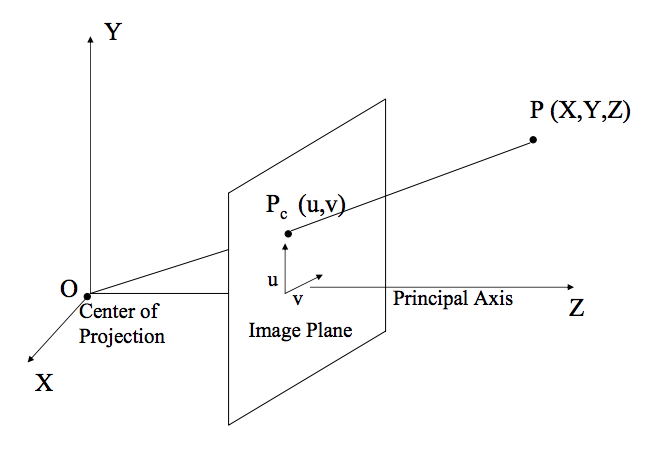
\includegraphics[width=7cm]{images/chapter4_pinhole_model.png}
  \end{center}
  \caption{Pinhole model \cite{website:majumder}.}
  \label{fig:pinhole}
\end{figure}

The projection matrix used is the union of the intrinsic and extrinsic camera parameters, which are defined via the calibration process. In this occasion, no calibration was required as the RGB-D sensor was already calibrated by default at the factory level and the required matrices were made available in TIAGO through a ROS topic.

The \textbf{PinHoleCameraModel} library available in Python was used to obtain the image plane 3D ray, determined by the u and v coordinates in Figure \ref{fig:pinhole}. However, before using the projection routine an initial camera info initialisation is needed. A subscription is therefore made to the \textbf{/xtion/rgb/camera\_info} whose callback calls the \textbf{fromCameraInfo} set-up routine where the camera's matrices including the distortion and projection ones are passed to the PinHoleCameraModel instance defined in the constructor.

Once the initialisation is complete, the 3D ray can be found by simply calling the \textbf{projectPixelTo3dRay} routine which takes as an argument a tuple, containing the coordinates of the RGB pixel to be projected, in this case the centre of the bounding box of the detection, with the first entry being the y coordinate and the second entry the x coordinate. The returned point is then used to find the ultimate 3D point.

\subsection{3D conversion}

All of the required data for the correct 3D pose estimation of the detection are known at this stage. Mainly the image plane coordinates and the depth, which aggregated together by using a ROS \textbf{Pose} message, gives the 3D vector point with respect to the RGB optical frame. However, the real interest is in knowing the 3D point with respect to the map, as this can then be used to send navigation commands followed by possible interaction features. Therefore, a further step is required.

This consists in using spatial transformations to find the rotation matrix which multiplied by the \textbf{PointStamped} transformed 3D point vector yields the map coordinate of the person. The \textbf{PointStamped} message is the same as the \textbf{Pose} message with the addition of a standard ROS header containing a stamp and frame\_id field required for the spatial transformation, and which have respectively been populated with the latest time and the original coordinate frame of the 3D point, in this case \textbf{xtion\_rgb\_optical\_frame}, as follows:

\begin{lstlisting}
transformHeader = Header()
transformHeader.stamp = rospy.Time(0)
transformHeader.frame_id = "xtion_rgb_optical_frame"
\end{lstlisting}

Finally, the \textbf{transformPoint} routine available in the \textbf{tf} module is used to convert the 3D point from one coordinate frame to another. The routine takes two arguments, the first one is the target coordinate frame, in this case \textbf{/map}, while the second one is the point to be converted, the PointStamped instance. The original coordinate frame to transform from is contained in the 3D PointStamped instance passed, and is going to be extracted from its header by the routine itself, hence why it was needed to extend the Pose message to a PointStamped one.

\subsection{Topic Message \& Markers}

Similarly to what was done with the two previous modules, the pose module computation is published over a topic called \textbf{poses} that would allow the user to subscribe to it and access the computed 3D detections' pose. Two custom messages were declared, a \textbf{Pose.msg} message that holds the single detection 3D location and a \textbf{Poses.msg} message that stores the 3D point locations. The messages definition of the Pose.msg(left) and the Poses.msg(right) are shown below:

\begin{multicols}{2}
  \begin{itemize}
    \item int32 ID
    \item Point pose
  \end{itemize}

  \columnbreak

  \begin{itemize}
    \item Header header
    \item Pose[] array
  \end{itemize}
\end{multicols}

The Pose.msg fields consists in a 32bits identifier that links the 3D pose to the corresponding detection and a Point field, which is a standard ROS message containing the x, y and z coordinates of the 3D pose as a standard 64bit floating point number. Finally the Poses.msg message has two fields, a header storing the usual time-stamp of the message creation and a list of type Pose that holds all the different Pose.msg instances. Populating these message follows the exact same rules and logic as the ones showed in previous chapters.

Visual markers were used as well to show the detections' pose on RVIZ. To create a marker for each detection, the standard ROS Marker was instantiated in the \textbf{createMarker} helper function defined in the \textbf{pose\_finding.py} script, where several fields were populated, including colour, scale and marker's coordinates among others. Moreover, for the message to be visualised in RVIZ, the message had to be specifically published over the \textbf{visualization\_marker\_array} topic as a \textbf{MarkerArray} type, hence the created markers had to be aggregated together. The following is a screen-shot showing how the marker are visualised on RVIZ.

\begin{figure}[H]
  \begin{center}
    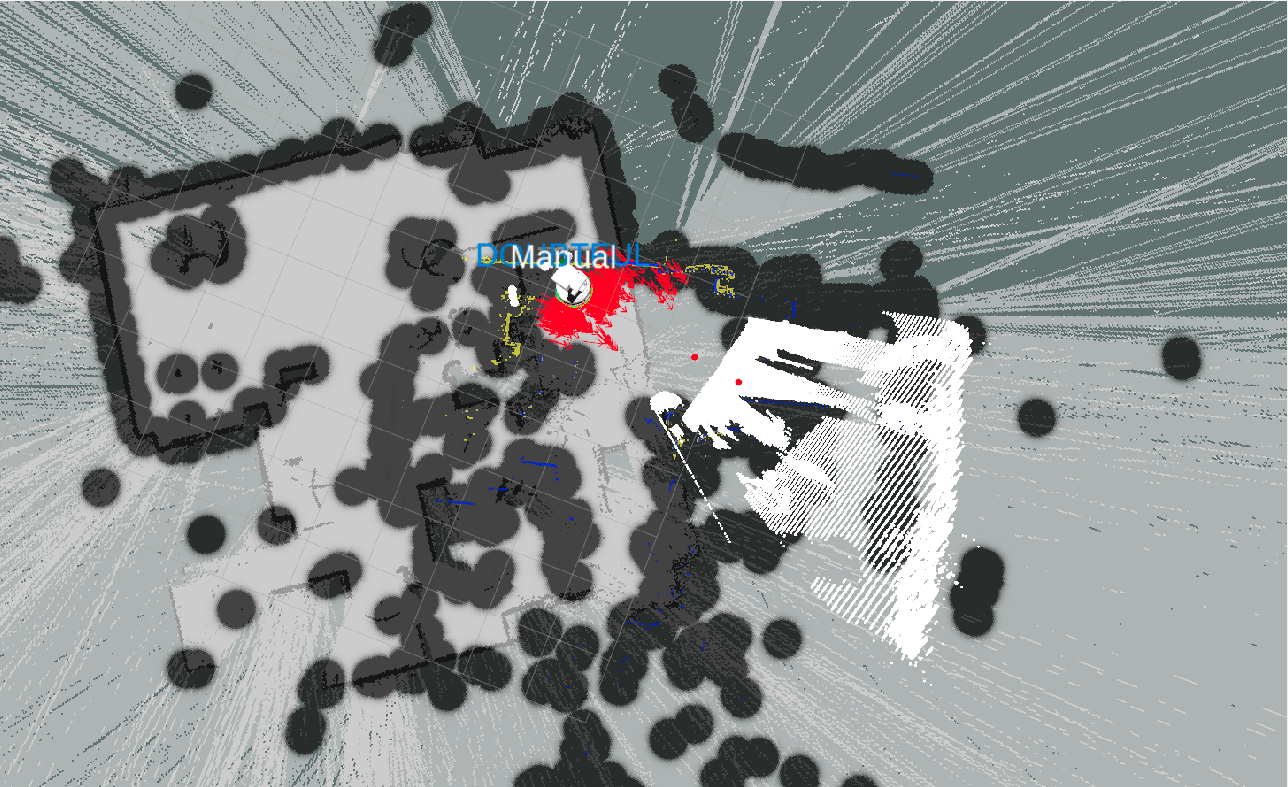
\includegraphics[width=.9\linewidth]{images/chapter4_markers.png}
  \end{center}
  \caption{RVIZ markers (red dots).}
  \label{fig:markers}
\end{figure}